\documentclass[12pt, titlepage]{article}
% \usepackage[bottom = 5cm, top = 5cm, left = 3cm, right = 3cm]{geometry}
\usepackage[margin = 1in]{geometry}
\usepackage[english]{babel}
\usepackage[utf8]{inputenc}
\usepackage[table]{xcolor}
\usepackage{graphicx, booktabs, tikz, csquotes, subcaption, enumitem, dcolumn, pdfpages, amsmath}
\usepackage[font=normalsize]{caption}%,labelfont=bf

\usepackage{endnotes}
\let\footnote=\endnote

\renewcommand*\rmdefault{ppl}

\usepackage{setspace}
\setstretch{1.5}

\usepackage[]{titlesec}
    \titleformat*{\section}{\large\bf}
    \titleformat*{\subsection}{\normalsize\it}

% Bibliography
% \usepackage[natbibapa]{apacite}
\usepackage[round]{natbib}
% \renewcommand{\bibliographytypesize}{\normalsize}
\setlength{\bibsep}{5pt}

% Cross-referencing with appendix
% (https://www.overleaf.com/learn/how-to/Cross_referencing_with_the_xr_package_in_Overleaf)
\makeatletter
\newcommand*{\addFileDependency}[1]{% argument=file name and extension
  \typeout{(#1)}
  \@addtofilelist{#1}
  \IfFileExists{#1}{}{\typeout{No file #1.}}
}
\makeatother

\newcommand*{\myexternaldocument}[1]{%
    \externaldocument{#1}%
    \addFileDependency{#1.tex}%
    \addFileDependency{#1.aux}%
}

% Cross-refs
\usepackage{xr-hyper}
\myexternaldocument{appendix}
\usepackage[colorlinks = TRUE, allcolors = blue]{hyperref}

\widowpenalty=10000
\clubpenalty=10000

\title{\Large Do TJ policies cause backlash?\\Evidence from street name changes in Spain}
\author{}
% \author{Francisco Villamil\footnote{Juan March Institute--Carlos III University of Madrid} \and Laia Balcells\footnote{Georgetown University}}
\date{\today}

% for word counting --------
%\usepackage[none]{hyphenat}
%\usepackage[nomarkers]{endfloat}
% --------------------------

\begin{document}

\maketitle

\begin{abstract}
\setstretch{1.2}\noindent
Memories of old conflicts often shape domestic politics long after these conflicts end. Contemporary debates about past civil wars and/or repressive regimes in different parts of the world suggest that these are sensitive topics that might increase political polarization, particularly when transitional justice policies are implemented and political parties mobilize discontentment with such policies. One such policy recently debated in Spain is removing public symbols linked to a past civil war and subsequent authoritarian regime (i.e., Francoism). However, the empirical evidence on its impact is still limited. This article attempts to fill this gap by examining the political consequences of street renaming. Using a difference-in-differences approach, we show that the removal of Francoist street names has contributed to an increase of electoral support for a new far-right party, Vox, mainly at the expense of a traditional right-wing conservative party, PP. Our results suggest that revisiting the past can cause a backlash among those ideologically aligned with the perpetrator, and that some political parties can capitalize on this.

\vspace{10pt}\noindent
\textbf{Keywords:} transitional justice, voting, conflict memories, Spain

\vspace{10pt}
\noindent
% \textbf{Keywords:} transitional justice, voting, conflict memories, Spain

\end{abstract}
\setstretch{1.5}

\newpage
\section*{Introduction}

Memories of contested historical events shape domestic politics across the world. One way in which historical memory is formed and reproduced is through symbols such as statues or street names, and their establishment (or removal) constitutes a policy that is often related to Transitional Justice (TJ) processes in societies emerging from authoritarian or conflicted pasts. These forms of so-called ``symbolic TJ policies'' are considered important to facilitate national reconciliation.

% and the public display of a contentious past related to the Civil War and slavery.
%Removing these symbols, a transitional justice (thereafter, TJ) policy, is defended on the grounds that they represent ideas that are no longer acceptable and constitute a roadblock to reconciliation.

Yet, symbol policies are not free of controversy. In Ukraine, removing Soviet statues during the `Leninopad' caused a backlash among sympathizers of the old Soviet regime \citep{Rozenas:2021}. In the South of the United States, there have been several instances of right-wing or white supremacist protests when statues of Confederates have been torn down, and there is a heated policy and scholarly debate about whether these statues should remain in public spaces or not \citep{Grossman:2016}.
%In some cases, these protests have turned violent.
%The 2017 `Unite the Right' rally in Charlottesville, Virginia, opposing the removal of a Robert E Lee statue, escalated into violence and resulted in the death of one person when a white supremacist drove his car into a crowd of counter-protesters.

%In Germany, the co-leader of Alternative for Germany (AfD) dubbed the Berlin Holocaust Museum a ``monument of shame'' \citep{Laub:2018aa}. In Poland, the right-wing Law and Justice (PiS) party has recently changed the National Memory Law, ``threatening to prosecute anyone claiming that the Polish Nation was responsible for Nazi crimes'' \citep[][183]{Zubrzycki:2020aa}.

In this study, we explore whether symbolic TJ policies cause a backlash. If yes, what are the political consequences of such backlash? Social movements or political parties can capitalize on grievances about the removal of symbols of a past regime to build further support. We probe into a potential backlash effect of the removal of public symbols linked to the Francoist regime in Spain, where memories of this dictatorship are divisive and potentially polarizing \citep{Balcells:2012aa}.
Our design exploits some of the changes brought about in Spain by the 2007 Law of Historical Memory (LHM), which introduced a mandate to remove Francoist symbols from public spaces, including street names. We examine whether street renaming generated an increase in electoral support for Vox, a relatively new far-right party that is gaining ground in Spain.

Traditional conservative parties in Spain have generally opposed TJ policies and have been adamant about sticking to the `pact of forgetting' that characterized the transition to democracy in the late 1970s \citep[e.g.][]{Fuente:1980aa}.
Yet, the Spanish far-right is more resolute in exonerating the Francoist regime and defending its memory.
In response to recent TJ policies promoted by a left-wing government, Vox has fiercely tried to capitalize on discontentment among Spaniards who do not support such policies.\footnote{Originated in 2013 from a split in the traditional right-wing party PP (Partido Popular), Vox promotes a discourse based on authoritarian conservatism and a hard-line version of Spanish nationalism. It shares with other populist right-wing parties in Europe a nativist ideology and a rejection of immigration, gender policies, and the social welfare state \citep{Turnbull-Dugarte:2019aa, Turnbull-Dugarte:2020aa}.} This party has been vocally opposed to the removal of Francoist symbols from public spaces or to the transfer of Francisco Franco's remains from the Valley of the Fallen's mausoleum to a private grave \citep{Taladrid:2019aa}. Vox has characterized the LHM as an instrument of leftist propaganda, has claimed that Spain's national unity is the path to overcome historical divisions, and has unabashedly whitewashed Francisco Franco's figure. However, we do not know whether this strategy has electorally benefited Vox or not, and identifying causality is thorny because of confounding events. For example, during the 2017 secessionist crisis in Catalonia, Vox was actively involved in the judicial prosecution of separatist leaders, posing as the true guarantor of Spanish territorial unity. The latter probably had an impact on its territorial performance in the 2019 elections.

%We aim to shade some light on this question.
%Originated from a split within the mainstream right-wing party (Partido Popular), Vox represents a hard version of Spanish nationalism.
%Its discourse glorifies Spain's imperial past and its national unity.
%It also condemns peripheral nationalisms and any attempt at redressing the official memory imposed by the Franco regime.
%In this study, we probe whether the removal of Francoist street names accounts for variation in support for Vox.
%Our results support the backlash hypothesis.
%Cross-sectional analyses show there is a correlation between the removal of Francoist street names and electoral support for Vox in Spanish 2019 elections.
%Also, in order to get closer to a causal identification,
We implement a difference-in-differences (DiD) design where we analyze the impact of Francoist street renaming on the growth in Vox's electoral support between 2016 and 2019.
%Focusing only on a subset of municipalities that still had Francoist street names in June 2016,
We find that support for Vox increased around 6\% more in municipalities where there was a Francoist street renaming between June 2016 and April 2019 than in places without such replacements. Support for the Partido Popular (PP) decreased 8\% more in those same municipalities, while support for the socialist party (PSOE) did not vary. This finding suggests a potential effect of these removals to increased asymmetric polarization, where only one sector of society (in this case, the right) radicalizes.
%While they cannot directly generalize due to the role of contextual factors, our findings have implications about symbolic TJ and other historical memory polices in other parts of the world.

%The politics of memory and the revision of a country's history are key issues in contemporary politics.
%National traditions and symbols across the world are being criticized because of their racial or ideological overtones.
%Even though those who support these revision policies usually claim that they promote reconciliation, our argument is that can also have the unintended side effect of increasing political polarization.

\section*{The effects of ``symbolic'' TJ policies}

After regime transitions or violent episodes, countries face the need to come to terms with the past \citep{Elster:2004aa}. To this end, countries often rely on different TJ policies, such as trials, truth commissions, reparations, amnesties, or ``symbolic'' measures like museums or memorials \citep{De-Brito:2001aa, Elster:2004aa, Balasco:2013aa}. All these various measures aim to serve justice, redress grievances, and reduce the probability of conflict recurrence \citep{Loyle:2017aa}. However, the short-term and long-term and consequences of TJ policies are still not clear.

Many scholars praise TJ policies, arguing that they increase the prospect for democracy \citep{Elster:2004aa, Sikkink:2007aa} and reduce the risk of future conflict by increasing accountability for past victimization \citep{Kim:2010aa, Meernik:2010aa} and redressing grievances \citep{Akhavan:1998aa, Loyle:2017aa}. Other authors posit that the positive view on TJ policies is overly optimistic and that there is scant evidence supporting a beneficial effect \citep{Mendeloff:2004aa, Thoms:2010aa}. Some even claim that TJ policies can harm reconciliation and conflict because they can renew social tensions in divided societies \citep{Snyder:2004aa}.
%\footnote{The idea that TJ policies might intensify old hatreds and divisions was precisely one of the arguments held by conservative sectors in Spain against the 2007 Law of Historical Memory.}
%Indeed, the debates about the past related to these TJ policies seem to have played a meaningful role in building a successful electoral discourse among populist right-wing parties in some European countries \citep{Martin:2020aa}.

%Previous research has paid close attention to the formal justice mechanisms of TJ policies, but we know much less about more informal measures of TJ and their effects on public opinion or voting behavior.
%Two recent works constitute a partial exception to this gap.
In an attempt to shed light on this debate, \cite{Capoccia:2020aa} study the impact of TJ trials on democratic attitudes in West Germany and find heterogeneous effects depending on the type of punishment and the group identity of the defendants. \cite{Balcells:2020aa}, for their part, study the impact of TJ museums with a field experiment in Santiago, Chile. They find that a single TJ museum visit can have reconciliatory and pro-democratic effects, and document no evidence of a backlash among those ideologically close to the Pinochet regime.

We aim to contribute to this literature by exploring the effects of a particular subset of TJ policies: removing symbols of a past regime from public spaces. We focus on Francoist street renaming in Spain. Just like the removal of statues and symbols, the building of museums or the establishment of historical markers \citep{Ward2021}, street renaming is a symbolic TJ policy \citep{Aguilar:2011aa}. Symbolic TJ intertwines with the politics of memory, which involve ``the shaping of collective memory by political actors and institutions'' \citep[][176]{Zubrzycki:2020aa}. While there has been significant research on other aspects of TJ policies such as trials, reparations, or lustration \citep{Nalepa:2010, Loyle:2017aa, voytas:2021}, the study of symbolic TJ is relatively underdeveloped.

In Spain, the 2007 LHM, promoted by a left-wing (PSOE) government, constituted an attempt to redress long-held grievances by the victims of the Nationalist side in the civil war (1936--1939) and the Francoist regime (1939--1977). It included provisions for the removal of Francoist symbols from public spaces, such as street names and monuments. Indeed, while many local governments had removed Francoist street names right after the transition to democracy, hundreds of municipalities had kept them because the historical memory issue was not salient or because local politicians deliberately avoided it.
The 2007 Law prompted municipal governments to be proactive and offered local associations a legal platform to pressure their local councils to remove Francoist symbols. Anecdotally, we know that these policies generated some backlash among Spanish right-wing citizens \citep[e.g.][]{Ezquiaga2021}. Yet, we do not know if this backlash was systematic or the extent to which it benefited the far-right, which tried to exploit it electorally. We test this hypothesis with local-level data.
%``backlash hypothesis'', namely, that removing public symbols will mobilize and radicalize those who are ideologically closer to these symbols. If this hypothesis is true, in the context of Spain, we would expect that the removal of Francoism symbols would lead to an increase in support for the far-right.

%\section*{Conflict memories and authoritarian backlash in Spain}

%We exploit two recent phenomena in Spanish politics: the consequences of the Law of Historical Memory and the recent rise of a far-right party, Vox.%, whose discourse rests heavily on the version of Spanish nationalism supported by Francoism.

%In Spain, the Law of Historical Memory (2007), promoted by a left-wing (PSOE) government, constituted an attempt to redress long-held grievances by the victims of the civil war and the Francoist regime. Among other things, it included provisions for the removal of Francoist symbols from public spaces, such as street names and monuments.

%Some local governments had already changed Francoist street names right after the transition to democracy.
%For instance, the \textit{Paseo de la Castellana} and the \textit{Avinguda Diagonal}, two of the main arteries of Madrid and Barcelona, respectively, were named \textit{Avenida del Generalísimo Franco} until 1979.
%However, these changes depended on an active decision made at the local level.
%In many places, either because the civil war/Francoist issue was less salient or because local politicians actively rejected the change, many streets were still named after Francoist symbols or leaders.
%The 2007 Law prompted local governments to act and offered local associations a legal platform to pressure their local councils.% to promote street name changes.
%\footenote{In fact, the Law of Historical Memory promoted and funded local `memory associations' that reviewed the local history and organized the exhumation of local mass graves.}

%These policies were hotly contested by particular sectors of Spanish society. By the late 2000s, even if the 2007 Law had a broad support in Spanish society, a significant proportion of the population still disagreed with its provisions \citep{Aguilar:2011aa}.
%Even from the very first years of democratic rule, rightist parties rejected the change of street names or the removal of public monuments by saying that revisiting history only brought old-seated divisions back \citep[e.g.][]{Fuente:1980aa}.
%\footnote{The exhumation of Francisco Franco from the Valley of the Fallen in late 2019 is probably the latest high-key example of the implementation of this law and the political tension it brought about \citep{Taladrid:2019aa}.}
%

%To analyze the effect of TJ policies aimed at removing symbols, we focus on electoral support for Vox as our measure for far-right ideological preferences.
%Vox is a relatively new party which promotes a discourse based on authoritarian conservatism and a hard-line version of Spanish nationalism. It originated in 2013 from a split in the traditional right-wing party (Partido Popular, or PP). It shares with other populist right-wing parties in Europe a nativist ideology and a rejection of immigration, gender policies, and the social welfare state \citep{Turnbull-Dugarte:2019aa, Turnbull-Dugarte:2020aa}.
%This discourse mirrors the `forgetting` policy developed by Franco in the postwar period \citep{Palomares:2004aa}.


%We make use of these two events to assess whether the politics of memory in Spain caused a backlash towards positions closer to the ideology of the Francoist regime. In particular, we measure whether the renaming of streets led to increased  support for Vox.
%Our expectation is that the relationship will be positive, supporting the backlash hypothesis.

\section*{Empirics}

We implement a DiD design analyzing the effect of Francoist street name removals on the growth in local electoral support for Vox between two different general elections in June 2016 and April 2019.
We focus on this period because Vox first participated in national elections in December 2015, and 2016--2019 is the only long enough electoral period in which it is possible to measure changes in its electoral share. Moreover, during this period, Vox experienced a surge in electoral support and turned into a critical electoral player in Spanish politics \citep{Turnbull-Dugarte:2020aa}.

We focus on all Spanish municipalities that still had at least one Francoist street name in June 2016. Our models aim to identify whether Vox electorally grew more in municipalities that renamed Francoist streets than in those that did not. % We discuss each of the variables below.

\subsection*{Francoist street name removal}

To build our main independent variable, we use data from the Spanish National Statistical Institute \citep{INE:2020aa} identifying all street names in Spain at different points in time. The INE offers data on all existing streets on June 30th and December 31st every year since 2010 (it also provides one-time data for June 2001).
Using the official ID number for each street, we can track name changes over time.

To identify streets named after Francoist symbols or figures, we use the list published by the Madrid City Council in 2017, following a report by a specially designated commission.\footnote{The full list is available online at https://bit.ly/37cLGgk (accessed 26/11/2020).} We expand it by including prominent Francoist names (e.g., `Jos\'e Antonio', `Calvo Sotelo', `Generalísimo', `General Franco') that the city of Madrid had already removed before 2017.\footnote{We show the full list in the Appendix (section~\ref{app:franc_names_list}).}
Our main variable is a binary indicator of Francoist street name removal between June 30th, 2016 and December 31st, 2018.\footnote{See section~\ref{app:treatment_strength} in the Appendix for more details about the coding.}

Figure~\ref{fig:changes_time} shows the number of Francoist street name removals during every six-month period since 2011. We can see that there is a spike after 2016, precisely during the period we examine. There are several reasons for this peak.
First, after the 2007 LHM, there were legal battles or lobbying campaigns to remove Francoist names, which dragged for some time and started to resolve after 2016. In mid-2016, Olmedo, Valladolid, became the first municipality to be sentenced for not complying with the 2007 LHM \citep{El-Norte-de-Castilla:2016aa}.
Second, after 2015, there was increased institutional activity in favor of street renaming, partly as a result of the PP losing grip of several municipal and regional governments in the 2015 elections \citep[e.g.][]{Vazquez:2016aa, El-Comercio:2016ab}.
We show more information on street name changes over time in the Appendix (section~\ref{app:descriptives_removals}).
%, such as Llanes, Asturias \citep{El-Comercio:2016aa}.
%Second, the decrease in votes for the mainstream right-wing party in the 2015 local and regional elections changed the balance of power which, together with a general increase in the salience of this issue, meant more institutional activity in this direction

\begin{figure*}[htb!]
\centering

  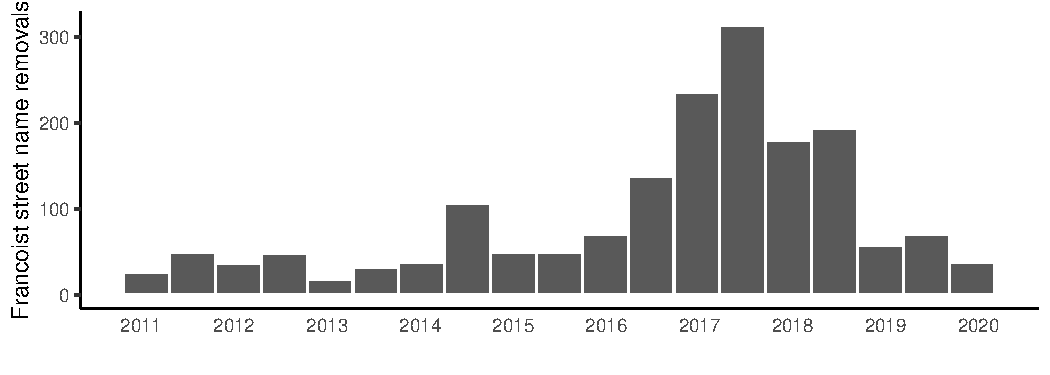
\includegraphics[width = 0.8\textwidth]{img/changes_by_year}

  \caption{Number of Francoist street name removals over time (2011-2020)}\label{fig:changes_time}

  \vspace{5pt}

  % \parbox[t]{0.84\textwidth}{\footnotesize{\textbf{Note:} Data from INE. After 2011, data was published every 6 months. Before that date, there is only one data point, in June 2001.}}

\end{figure*}

%The post-2016 increase could bias the results if related to political dynamics that also explained changes in political preferences.
%However, a closer look at the data shows that, in terms of voting patterns, there are no significant differences between municipalities that removed Francoist names during the 2016--2019 period and those that did not (see sections \ref{app:descriptives_removals} and \ref{app:treated_vs_control_vs_outsample} in Appendix). %Geographically, this post-2016 increase in Francoist street removals is mostly driven by relatively small municipalities in central regions of Spain.

%on street name removals and on which municipalities still had Francoist street names during this period suggests this is not the case (see sections \ref{app:descriptives_removals} and \ref{app:treated_vs_control_vs_outsample} in Appendix).
%We discuss at length the differences between municipalities in and out of the sample in the appendix (section~\ref{app:treated_vs_control_vs_outsample}).% we show that most of the municipalities that removed Francoist street names were small municipalities that had more Francoist street names to start with, and mostly in provinces in the central regions of Spain, which is in line with the factors discussed above.

\subsection*{Variables}

Our primary dependent variable is the percentage of electoral support for Vox.
We obtained the data from the Spanish Ministry of Interior\footnote{Results are available at \href{http://www.infoelectoral.mir.es/}{http://www.infoelectoral.mir.es/} (accessed 03/12/2020).}
and calculated the share of valid votes for Vox in each municipality in the 2016 and 2019 general elections.\footnote{See section~\ref{app:timeline_elections} in the Appendix for a timeline of elections in Spain.}

In addition, we also examine the electoral share of two mainstream parties, the Popular Party (\textit{Partido Popular}, PP), at the right, and the socialist party (\textit{Partido Socialista Obrero Español}, PSOE), at the left, to capture local shifts in political preferences.

We include a series of control variables at the local level.
In particular, we include turnout in the June 2016 elections, (logged) population from the 2011 census, the (logged) number of Francoist street names in June 2016, the unemployment rate in January 2016, and a binary indicator of whether a leftist mayor won the May 2015 municipal elections.
In addition, we also include fixed effects at the region level (Autonomous Communities).
We show summary statistics of all variables in the Appendix (section~\ref{app:descriptives}).

\subsection*{Models}

We run OLS regressions on the electoral support for Vox, PP, and PSOE in the June 2016 and April 2019 elections as dependent variables, using an indicator of Francoist street name removal between June 2016 and December 2018 as our main independent variable.
We define the DiD model as:

\begin{equation}
\begin{split}
    Y_{it} =&  \beta_0 + \beta_1 Removal_{i} + \beta_2 April2019_{t} +\\
    &\beta_3 (Removal_{i} \times April2019_{t}) + \beta^\top \mathbf{x}_{i} + \alpha_{r} + \epsilon_{it}
\end{split}
\end{equation}

Where $Y_{it}$ is the share of support for Vox in municipality $i$ and election $t$, $\mathbf{x}_{i}$ is a vector of covariates, $\alpha_{r}$ are region fixed effects, and $\epsilon_{it}$ is the error term.
The effect of street name removals is captured by $\beta_3$, the interaction between the $t_{1}$ (April 2019) and treatment (Francoist street name removal) indicators.

As argued above, we only examine municipalities that still had Francoist street names in June 2016. Table~\ref{tab:sample_trt} shows how many of them renamed Francoist streets during the period of study.
Moreover, we limit the sample to municipalities where Vox participated in June 2016.\footnote{Vox was a relatively new party in 2016 and did not field candidates in some provinces.}
In the Appendix, we include detailed information about the sample and both treatment and control groups (sections~\ref{app:descriptives}-\ref{app:treated_vs_control_vs_outsample}), and show models for PP and PSOE using the full sample (section~\ref{app:robustness_did}).

\begin{table}[!htbp] \centering
\caption{DiD sample classification}
\label{tab:sample_trt}
\small
\begin{tabular}{lcc}
\\[-1.8ex]\hline
\hline \\[-1.8ex]
\multicolumn{1}{p{3cm}}{\hspace{3cm} Francoist names} & \multicolumn{2}{p{3.5cm}}{Removed Francoist names, 2016--2018?}\\
in June 2016? & No & Yes \\
\cline{2-3} \\[-1.8ex]
No & 6455 & 0 \\
 & (100\%) & (0\%) \\
Yes (DiD sample) \hspace{2cm} & 1184 & 454 \\
 & (72\%) & (28\%) \\
\\[-1.8ex]\hline
\hline \\[-1.8ex]
\multicolumn{3}{c}{\parbox[t]{0.55\textwidth}{\textit{Note:} Row percentages. Changes in 2016--2018 refer to the period between 01/07/2016 and 31/12/2018.}}\\
\end{tabular}
\end{table}


Focusing on municipalities that still had Francoist street names in 2016 implies that the DiD sample is more rightist than the average in Spain.\footnote{Municipalities that still had not changed Francoist names by late 2018 were portrayed as the `resistance' to the LHM \citep{Blanco-Elipe:2018aa}. Their dodging of the LHM was possible because of delays in the legal procedures or some form of `foot-dragging' by local authorities.}
In the Appendix, we compare municipalities in the sample to those out of the sample (section~\ref{app:treated_vs_control_vs_outsample}).

\section*{Results}

Table~\ref{tab:did_deco} shows the mean electoral share for each of the three parties in the 2016 and 2019 elections for the treated and control groups and the base difference in differences.
A first look shows that support for Vox between 2016 and 2019 increased, on average, 0.74 points more in municipalities that removed Francoist street names during that period than in those that did not, while support for PP and PSOE decreased 1.7 and 0.23 points more, respectively, in those same municipalities.

\begin{table}[!htbp] \centering
\caption{Mean electoral share in sample}
\label{tab:did_deco}
\small
\begin{tabular}{lccccccc}
\\[-1.8ex]\hline
\hline \\[-1.8ex]
\\[-1.8ex]
& \multicolumn{3}{c}{June 2016} & \multicolumn{3}{c}{April 2019} & \\\\[-1.8ex]
\cline{2-7}\\[-1.8ex]
Party & $Control$ & $Treated$ & $\Delta$ & $Control$ & $Treated$ & $\Delta$ & $\Delta_{2019} - \Delta_{2016}$ \\
\hline \\[-1.8ex]
Vox & 0.21 & 0.21 & 0 & 12.54 & 13.28 & 0.74 & 0.74 \\
PP & 41.22 & 46.77 & 5.55 & 23.83 & 27.68 & 3.85 & -1.7 \\
PSOE & 29.13 & 28.01 & -1.12 & 33.38 & 32.03 & -1.35 & -0.23 \\
\hline
\hline \\[-1.8ex]
\end{tabular}
\end{table}



To probe whether the differences above are statistically significant, we run regression models. Table~\ref{tab:main_did} presents the regression results, and figure~\ref{fig:main_did} shows the simulated DiD estimate of Francoist street renaming, using the models with control variables.


% Table created by stargazer v.5.2.2 by Marek Hlavac, Harvard University. E-mail: hlavac at fas.harvard.edu
% Date and time: Thu, May 27, 2021 - 17:29:25
% Requires LaTeX packages: dcolumn 
\begin{table}[!htbp] \centering 
  \caption{Francoist street name removal and increase in electoral support for parties} 
  \label{tab:main_did} 
\small 
\begin{tabular}{@{\extracolsep{-20pt}}lD{.}{.}{-3} D{.}{.}{-3} D{.}{.}{-3} } 
\\[-1.8ex]\hline 
\hline \\[-1.8ex] 
\\[-1.8ex] & \multicolumn{1}{c}{VOX} & \multicolumn{1}{c}{PP} & \multicolumn{1}{c}{PSOE} \\ 
\\[-1.8ex] & \multicolumn{1}{c}{(1)} & \multicolumn{1}{c}{(2)} & \multicolumn{1}{c}{(3)}\\ 
\hline \\[-1.8ex] 
 (Intercept) & -1.470^{**} & 56.375^{***} & 34.870^{***} \\ 
  & (0.451) & (0.922) & (0.876) \\ 
  Francoist street name removal & -0.132 & 1.158^{*} & -0.159 \\ 
  & (0.262) & (0.476) & (0.453) \\ 
  Election April 2019 & 12.319^{***} & -17.406^{***} & 4.629^{***} \\ 
  & (0.167) & (0.338) & (0.320) \\ 
  Francoist removal $\times$ April 2019 & 0.724^{*} & -1.405^{*} & -0.434 \\ 
  & (0.352) & (0.639) & (0.607) \\ 
 \hline \\[-1.8ex] 
Controls & \multicolumn{1}{c}{Yes} & \multicolumn{1}{c}{Yes} & \multicolumn{1}{c}{Yes} \\ 
CCAA Fixed Effects & \multicolumn{1}{c}{Yes} & \multicolumn{1}{c}{Yes} & \multicolumn{1}{c}{Yes} \\ 
Observations & \multicolumn{1}{c}{2,310} & \multicolumn{1}{c}{3,223} & \multicolumn{1}{c}{3,242} \\ 
R$^{2}$ & \multicolumn{1}{c}{0.768} & \multicolumn{1}{c}{0.720} & \multicolumn{1}{c}{0.482} \\ 
Adjusted R$^{2}$ & \multicolumn{1}{c}{0.766} & \multicolumn{1}{c}{0.717} & \multicolumn{1}{c}{0.478} \\ 
\hline 
\hline \\[-1.8ex] 
\multicolumn{4}{c}{\parbox[t]{0.75\textwidth}{\textit{Note:} $+ p<0.1; * p<0.05; ** p<0.01; *** p<0.001$. Only municipalities that had at least one street with a Francoist name in $t_{0}$ were included in the sample.}} \\ 
\end{tabular} 
\end{table} 


\begin{figure*}[htb!]
\centering

    \vspace{25pt}

  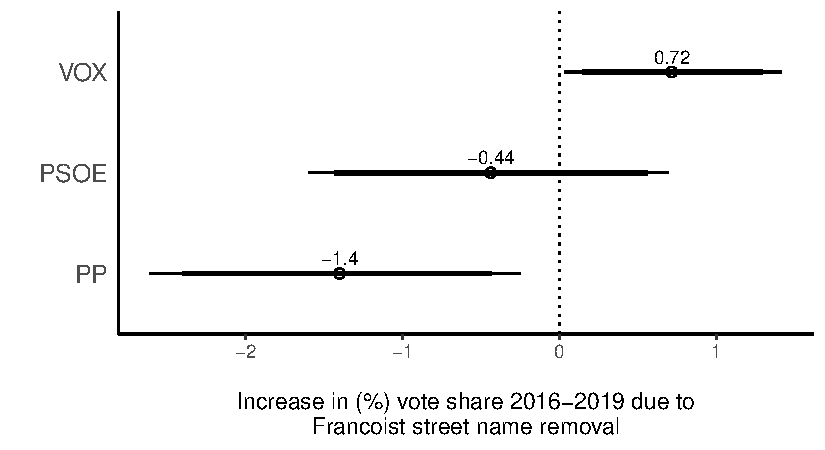
\includegraphics[width = 0.6\textwidth]{img/DiD_estimates}

  \caption{DiD estimates of Francoist street renaming on vote change, obtained from simulations (mean and 90\%/95\% CIs)}\label{fig:main_did}

\end{figure*}

The evidence is supportive of the backlash hypothesis. First, Vox increased its support 0.7 points more in municipalities that renamed Francoist street names than in those that did not. Considering that the nation-wide electoral share of Vox in April 2019 was 10.3\%, this effect is non-negligible: the change in electoral support was around 6\% higher in these municipalities.
Second, removing Francoist street names is related to a decrease in electoral support for PP, of almost 1.5 points. Interestingly, it does not significantly affect electoral support for PSOE, indicating that the change in political preferences takes place among rightist individuals. This last result is coherent with the idea that increased support for the far-right was linked not only to street renaming but to mobilization strategies of the far-right.

Our findings could be confounded if Francoist street renaming was driven by the same factors also explaining a shift to far-right preferences.
One possibility is that these street name changes took place in more conservative areas where Spanish nationalism was stronger.
In this case, we should see different trends before 2016 between municipalities that later removed Francoist street names and those that did not.
Figure~\ref{fig:par_trends_norm} shows normalized electoral trends among control and treated groups for PP and Vox.
Although data for Vox only goes six months back in time, there are no distinct trends for the two parties for which we find an effect of Francoist street renaming before June 2016.
We show data on pre-treatment trends in the Appendix (section~\ref{app:robustness_did}), even though a strict test of the parallel trends assumption is not possible given the absence of previous data on Vox, which emerged in 2014.

\begin{figure*}[htb!]
\centering

  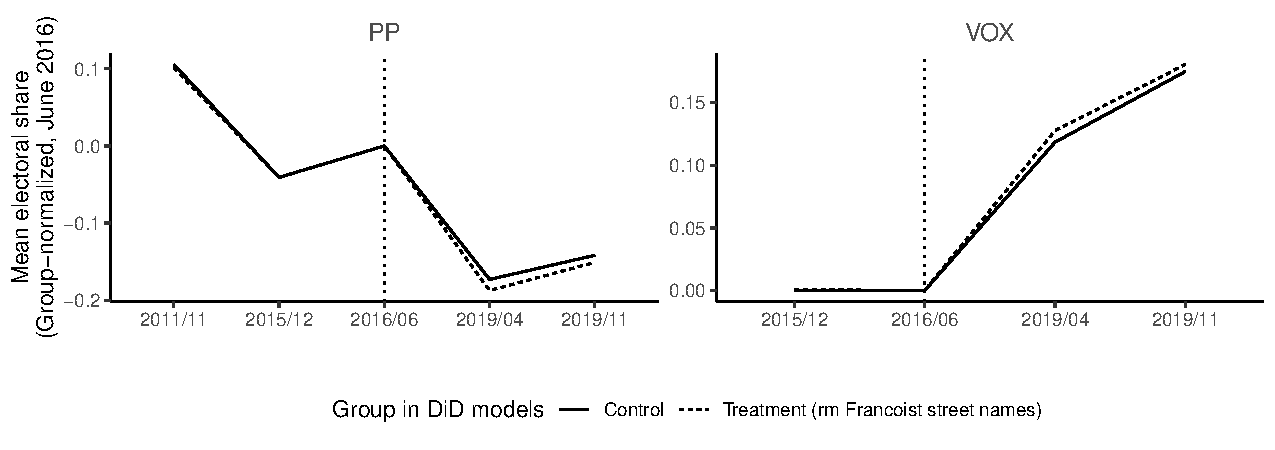
\includegraphics[width = \textwidth]{img/par_trends_norm}

  \caption{Pre- and post-treatment trends in Vox and PP electoral share}\label{fig:par_trends_norm}

\end{figure*}

In the Appendix, we include several additional analyses. We present cross-sectional models (section~\ref{app:crosssec}) using the independent variable in continuous form, tracking Francoist street name removals during different periods (including changes between 2001 and 2019), and using both support for Vox in the November 2019 elections as well as the change in support between April and November 2019 as dependent variables.
The results are coherent with the DiD analyses. They also show that Francoist street name removals account for Vox's growth between 2016 and 2019 but not for the changes between April and November 2019, which suggests that any local effect due to a backlash over the politics of memory took place mainly during the period we analyze.

Finally, we test the robustness of the DiD results to different specifications (section~\ref{app:robustness_did}), in particular: including the primary independent variable in continuous form (logged number of street name removals), excluding from the sample municipalities where Vox did not have any votes in 2016, and changing the independent variable so it also includes street renamings registered in the first half of 2019.
We also show results from first-difference models (section~\ref{app:first_diff}).
Results do not significantly change when using alternative specifications and support the main findings.

\section*{Conclusion}

Using local-level data, we analyze the political effect of Francoist street renaming in Spain and find evidence in favor of a backlash hypothesis. In the short-term, Francoist street name removals increase support for a far-right party, Vox, which has recently gained steam with a discourse grounded in an authoritarian and an exclusionary version of Spanish nationalism. Vox has grown in these places at the expense of the traditional conservative party, PP, but of the main left-wing party, PSOE, pointing to a process of asymmetric polarization resulting from this policy.

The results from our analyses echo recent debates about symbolic TJ policies and memories of past conflicts in other countries. Our goal is not to take a normative stand against these policies. Despite potential short-term backlash effects, we believe that they can be highly beneficial in the long run (these measures could well contribute to national reconciliation down the road). Moreover, TJ symbolic policies might have these unintended effects only where some political parties take electoral advantage of this issue. In other words, asymmetric polarization does not have to be an automatic outcome of these policies and actions of other political parties can perhaps palliate it. For example, by countering narratives or compensating the aggrieved in other ways (i.e., relocating these symbols into a museum), interested political and social actors could limit the extent to which this discontentment can be opportunistically exploited by more extreme parties. The extent to which such remedial policies can work is nonetheless out of the scope of this paper.

Finally, while we have focused on the removals of symbols, other TJ policies might not have similar backlash effects. For instance, recent research shows that TJ museums can promote reconciliation \citep{Balcells:2020aa}, and that reparations can increase political engagement among victims \citep{voytas:2021}. The average impact of TJ will depend on how the effects of the  different measures add up \citep{Olsen:2010aa, Loyle:2017aa}.
Overall, this article contributes to an open and lively scholarly debate on the effectiveness of TJ policies.

\newpage
\begingroup
\parindent 0pt
\parskip 2ex
\def\enotesize{\normalsize}
\theendnotes
\endgroup

\clearpage
\bibliographystyle{rap}
\bibliography{REF}

%\newpage
%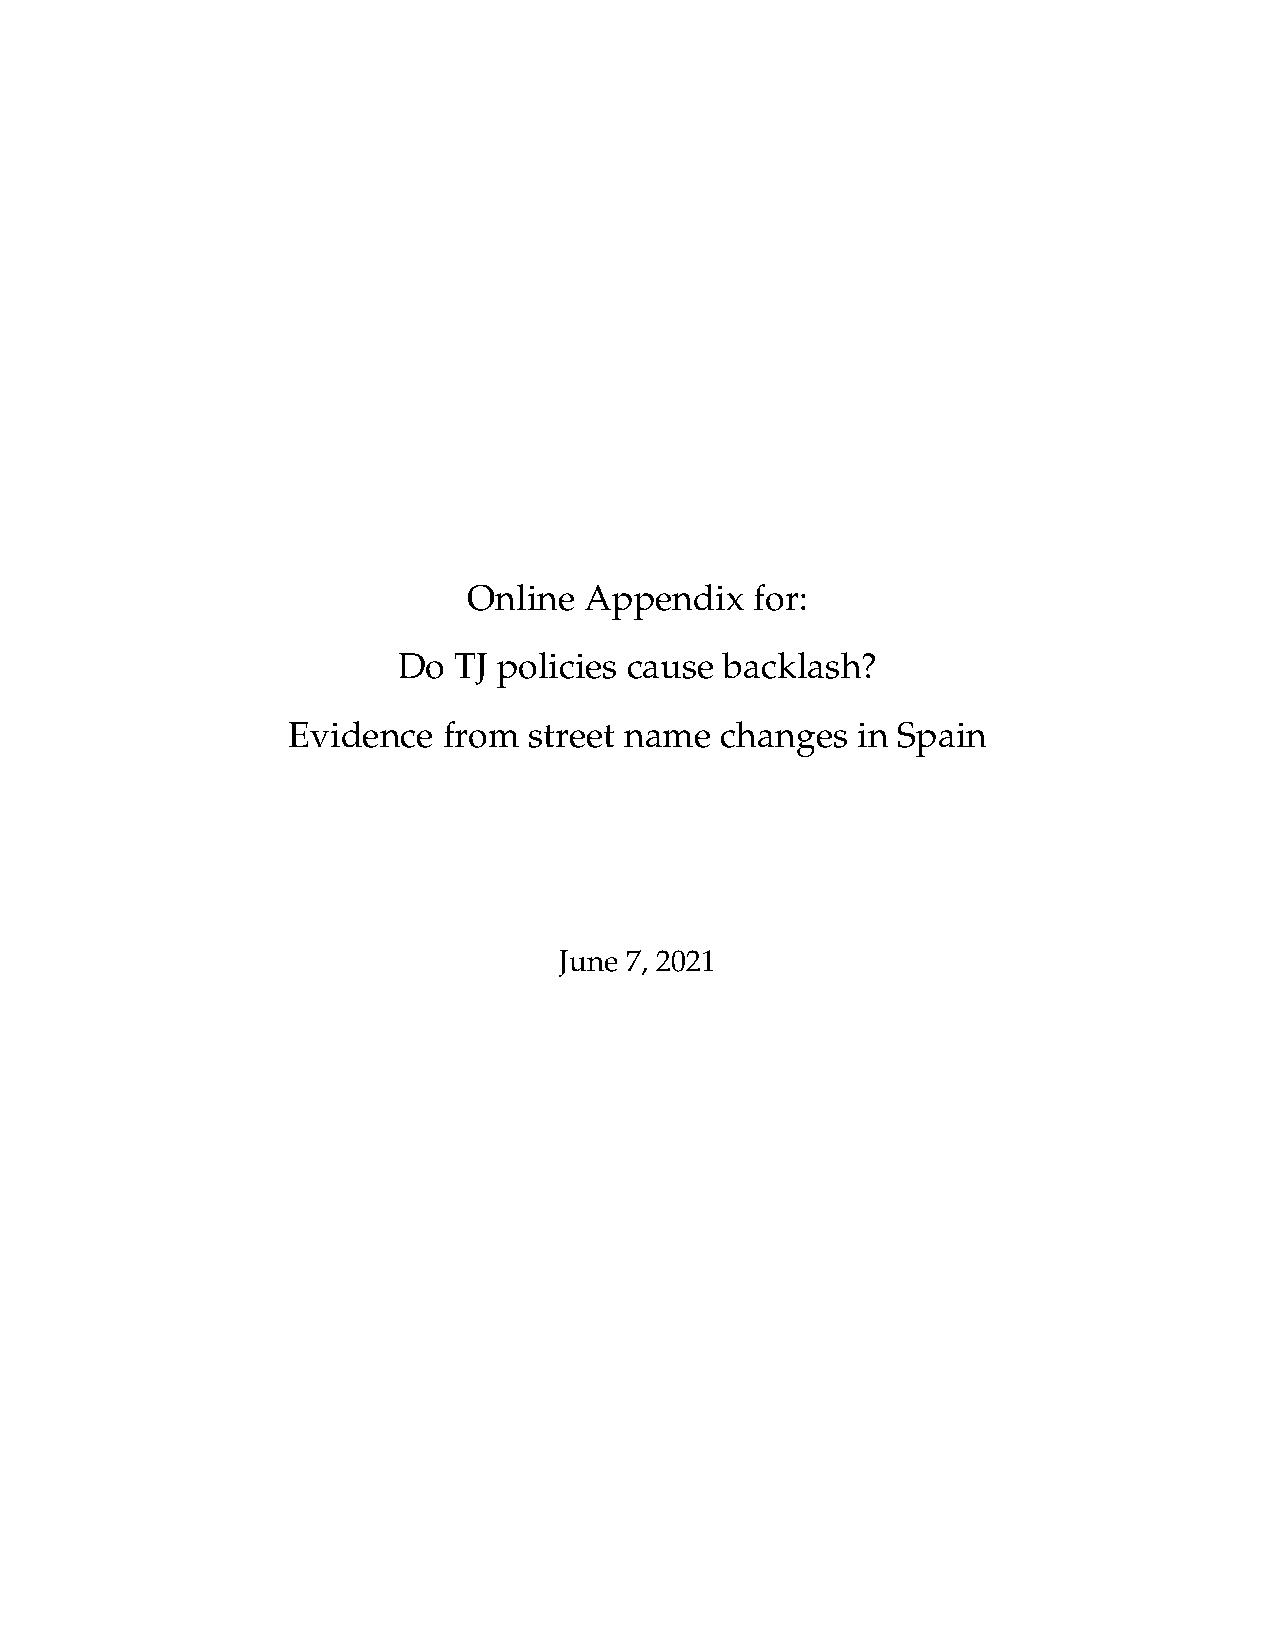
\includepdf[pages=-]{appendix.pdf}

\end{document}
